\documentclass[conference]{IEEEtran}

\usepackage{amsmath,amssymb,amsfonts}
\usepackage{graphicx}
\usepackage{textcomp}
\usepackage{xcolor}
\definecolor{linkblue}{RGB}{95,155,235}
\usepackage[normalem]{ulem}
\usepackage[colorlinks=true,urlcolor=linkblue,linkcolor=black]{hyperref}

\graphicspath{{./}}
\Urlmuskip=0mu plus 1mu\relax

\begin{document}

\title{Personal Finance Tracker and Analyzer}

\author{%
\textbf{Student Project Team}\\
Maria Davydova, Maxim Ivanov, Alexey Mikhailenko, Nikolay Tagin\\
\href{https://github.com/taginnikolaj/Personal-finance-tracker}{\textcolor{linkblue}{\uline{https://github.com/taginnikolaj/Personal-finance-tracker}}}%
}

\maketitle

\begin{abstract}
This report presents the Personal Finance Tracker and Analyzer project, a tool for automated accounting of personal expenses with support for manual input, downloading data from files, OCR receipt recognition, and visualization of financial statistics. The project is implemented in Python using the libraries pandas, matplotlib, requests and others. The system allows users to analyze their expenses by category, day, and month, as well as track spending against category budgets. The solution is aimed at helping people improve financial discipline and reduce stress associated with unaccounted expenses.
\end{abstract}

\section{Introduction}
The modern rhythm of life often leads to people losing control of their finances. The lack of daily expense tracking leads to overspending, poor budgeting, and financial stress. Existing solutions such as Excel or mobile applications either require manual work or are too complex for beginners. Our project offers a simple, flexible, and automated Python-based solution that can be easily expanded to add AI, API, and new features. The goal is to provide the user with an intuitive interface for analyzing their expenses without having to be a programmer.

\section{Problem Statement}
People need a simple, accessible way to track, analyze, and understand their personal finances.

The objectives of the project are:
\begin{itemize}
\item to provide the possibility of manually entering transactions;
\item to support downloading data from CSV and JSON files;
\item to implement the deletion of erroneous records;
\item to add the receipt recognition function via OCR;
\item to provide analysis tools: statistics, categorization, and trends;
\item to visualize data in the form of graphs and tables;
\item to make the system extensible and convenient for further development.
\end{itemize}

\section{Existing Work}
There are various financial accounting applications on the market:
\begin{itemize}
\item Excel / Google Sheets require manual entry of formulas and are prone to errors.
\item Mobile applications are closed systems with limited functionality and paid subscriptions.
\item Python libraries such as finance-tracker and budget-app often do not have a GUI and require programming knowledge.
\end{itemize}

Our solution combines the advantages of all approaches: automation as in Excel, flexibility as in Python, ease of use as in mobile applications, but free and open.

\section{Objectives and Scope}
\textbf{Objectives:}
\begin{itemize}
\item Create a working prototype of an expense tracker.
\item Implement basic functions: input, download, analysis, and visualization.
\item Integrate OCR for automatic data entry from receipts.
\item Ensure the readability of the code and the possibility of its extension.
\end{itemize}

\textbf{Scope:} personal use for budget control.

\section{Requirements}
\subsection{Functional Requirements}
\begin{itemize}
\item The ability to manually enter transactions: date, amount, category, and description.
\item Downloading data from CSV and JSON files.
\item Deleting transactions by ID.
\item Receipt recognition via OCR.
\item Automatic calculation of statistics: total amount, average, min/max, and quantity.
\item Grouping expenses by categories and dates.
\item Charting: pie chart, bar chart, line chart, and histogram.
\item Displaying results in tables and graphs.
\item Category budget management with budget vs actual reporting.
\end{itemize}

\subsection{Non-functional Requirements}
\begin{itemize}
\item The code should be readable and well documented.
\item The program should work in a standard Python environment without complex installations.
\item It should be possible to easily add new functions such as API, ML, and web interface.
\item The output interface should be understandable even for non-programmers.
\item Error handling is required when entering data and working with the API.
\end{itemize}

\section{Approach and Design}
\subsection{Project Architecture}
The project is implemented on a modular basis, which ensures a clear separation of responsibilities between components and simplifies code maintenance.

\textbf{Main modules:}
\begin{itemize}
\item The data model is a \texttt{Transaction} class that describes a single financial transaction.
\item The managing component is the \texttt{FinanceManager} class, which is responsible for storing, processing, and analyzing all transactions.
\item Configuration settings provide a centralized settings block for controlling program behavior without modifying core code.
\item Auxiliary functions provide utilities for searching files, parsing user input, and error handling.
\item The OCR module provides integration with an external API for recognizing receipts.
\item The visualization module is responsible for construction of graphs based on the processed data.
\end{itemize}

This architecture allows independently testing and developing each component, as well as easily adding new functions.

\subsection{Technology Selection}
\begin{itemize}
\item Programming language: Python 3.x.
\item Runtime environment: Python environment with notebook support.
\end{itemize}

\textbf{Main libraries:}
\begin{itemize}
\item \texttt{pandas} for storing, filtering, and aggregating tabular data.
\item \texttt{matplotlib} for building static graphs such as pie charts, bar charts, line charts, and histograms.
\item \texttt{requests} for sending HTTP requests to an external OCR API.
\item \texttt{csv} and \texttt{json} as standard modules for reading and writing data in popular formats.
\item \texttt{re} for using regular expressions when parsing text from receipts.
\item \texttt{pathlib} for convenient and cross-platform work with file paths.
\end{itemize}

All dependencies are standard or easily installed via \texttt{pip}, which makes the project portable and reproducible.

\subsection{Class Design}
\begin{itemize}
\item \textbf{Transaction Class.} The class represents a model of a single financial transaction. It encapsulates the transaction data and ensures its validation. The \texttt{validate\_date()} and \texttt{validate\_amount()} methods ensure that the date matches the \texttt{YYYY-MM-DD} format, and the amount is a positive number. This prevents incorrect data from entering the system. The \texttt{to\_dict()} method is also implemented, which converts an object into a dictionary, which is convenient for saving in JSON or displaying in a table.
\item \textbf{FinanceManager Class.} This class is the central control component of the system. It stores a list of all transactions and provides methods for working with them. The class supports loading data from CSV and JSON files, adding transactions manually, deleting by index, as well as calculating key metrics and grouping data for analysis.
\item \textbf{OCR Module.} An external OCR-Space service is used to automate data entry from paper receipts. The module consists of two main functions:
\begin{itemize}
\item \texttt{call\_ocr\_space(image\_path, api\_key, language='auto')} sends the receipt image to the OCR-Space server via a POST request and receives a JSON response with the recognized text.
\item \texttt{parse\_receipt\_items(ocr\_result)} analyzes the response from the API: it extracts rows with product names and prices, matches them by vertical position, ignores service words such as total, tax, and subtotal, and returns a DataFrame with columns \texttt{description}, \texttt{amount}, and \texttt{category}.
\end{itemize}
\end{itemize}

\section{Implementation}
\begin{itemize}
\item \textbf{Setting up the environment and importing libraries.} At the initial stage, the necessary Python libraries were connected to work with data, the file system, and graphics. Special attention is paid to configuring visualization styles and limiting the number of output rows in tables to avoid overloading the interface with unnecessary information.
\item \textbf{Development of the Transaction class.} The Transaction base class was created, representing a single financial transaction. The key feature of this class is the implementation of strict validation of input data. The \texttt{validate\_date()} method ensures dates follow the \texttt{YYYY-MM-DD} format, while \texttt{validate\_amount()} guarantees positive numeric values. The \texttt{to\_dict()} method provides convenient conversion for display and serialization.
\item \textbf{Development of a management class (FinanceManager).} The central element of the architecture is the FinanceManager class, which aggregates all transactions and provides comprehensive tools for working with them.
\item \textbf{System settings.} For the convenience of the user, a separate configuration block has been allocated, allowing flexible control of the program without changing the main code.
\item \textbf{Auxiliary utilities.} A set of auxiliary functions has been developed to automate routine tasks:
\begin{itemize}
\item File search: automatically search for files using preferred names or standard patterns.
\item Input parsing: converts comma-separated text lines into structured transaction data.
\item ID processing: reads and validates a list of transaction identifiers for deletion.
\end{itemize}
\item \textbf{Loading and clearing data.} A data processing pipeline is implemented: at startup, the system automatically attempts to load existing files (CSV or JSON). After loading, manual records from the settings are added, and then transactions specified for deletion are removed by ID. All changes are immediately reflected in the current data table with proper indexing.
\item \textbf{Integration of optical recognition (OCR).} To automate data entry from paper media, a module for working with the external API of the OCR-Space service has been implemented:
\begin{itemize}
\item Sending the request: \texttt{call\_ocr\_space()} sends the receipt image to the processing server with appropriate API key and language settings.
\item Response parsing: \texttt{parse\_receipt\_items()} analyzes the received text using spatial coordinates from the OCR result. The algorithm matches product descriptions, typically on the left side of the receipt, with corresponding prices, typically on the right side, by comparing vertical positions. Service labels such as total, tax, and subtotal are ignored. Dates and other non-item lines are filtered out.
\end{itemize}
\item \textbf{Receipt processing.} A complete receipt reading scenario is implemented: if OCR is enabled in the settings, the system finds the image file, sends it for recognition, parses the results, and automatically adds the recognized items to the general database of transactions with the current date or a specified date from settings. Error handling is provided: if recognition fails or the receipt file is not found, the program continues execution without interruption.
\item \textbf{Final analysis and reporting.} At the final stage, the data is aggregated and displayed in a convenient way:
\begin{itemize}
\item A complete table of all transactions with assigned IDs after applying filters.
\item A block of main statistics: total expenses, average receipt amount, maximum and minimum purchases.
\item Detailed breakdown of expenses by category with percentage of total.
\item Daily, weekly, and monthly totals tables for tracking spending dynamics over different time horizons.
\item Budget report comparing actual spending against user-defined category budgets with status indicators.
\end{itemize}
\item \textbf{Data visualization.} A comprehensive unified dashboard is constructed to visually represent the results:
\begin{itemize}
\item Category totals bar chart (horizontal): shows absolute amounts of expenses by category, sorted descending for easy comparison.
\item Pie chart: displays the share of each category in total expenses.
\item Budget vs actual bar chart: compares actual spending against category budgets, with visual indicators for overspending.
\item Daily trend line chart: shows the change in daily expenses over time, allowing identification of spending patterns.
\item Weekly summary bar chart: aggregates expenses by week for broader trend analysis.
\item Monthly summary bar chart: shows spending patterns across months.
\item Transaction amount distribution histogram: illustrates the frequency of transaction amounts, with the mean value highlighted.
\end{itemize}
\end{itemize}

\begin{center}
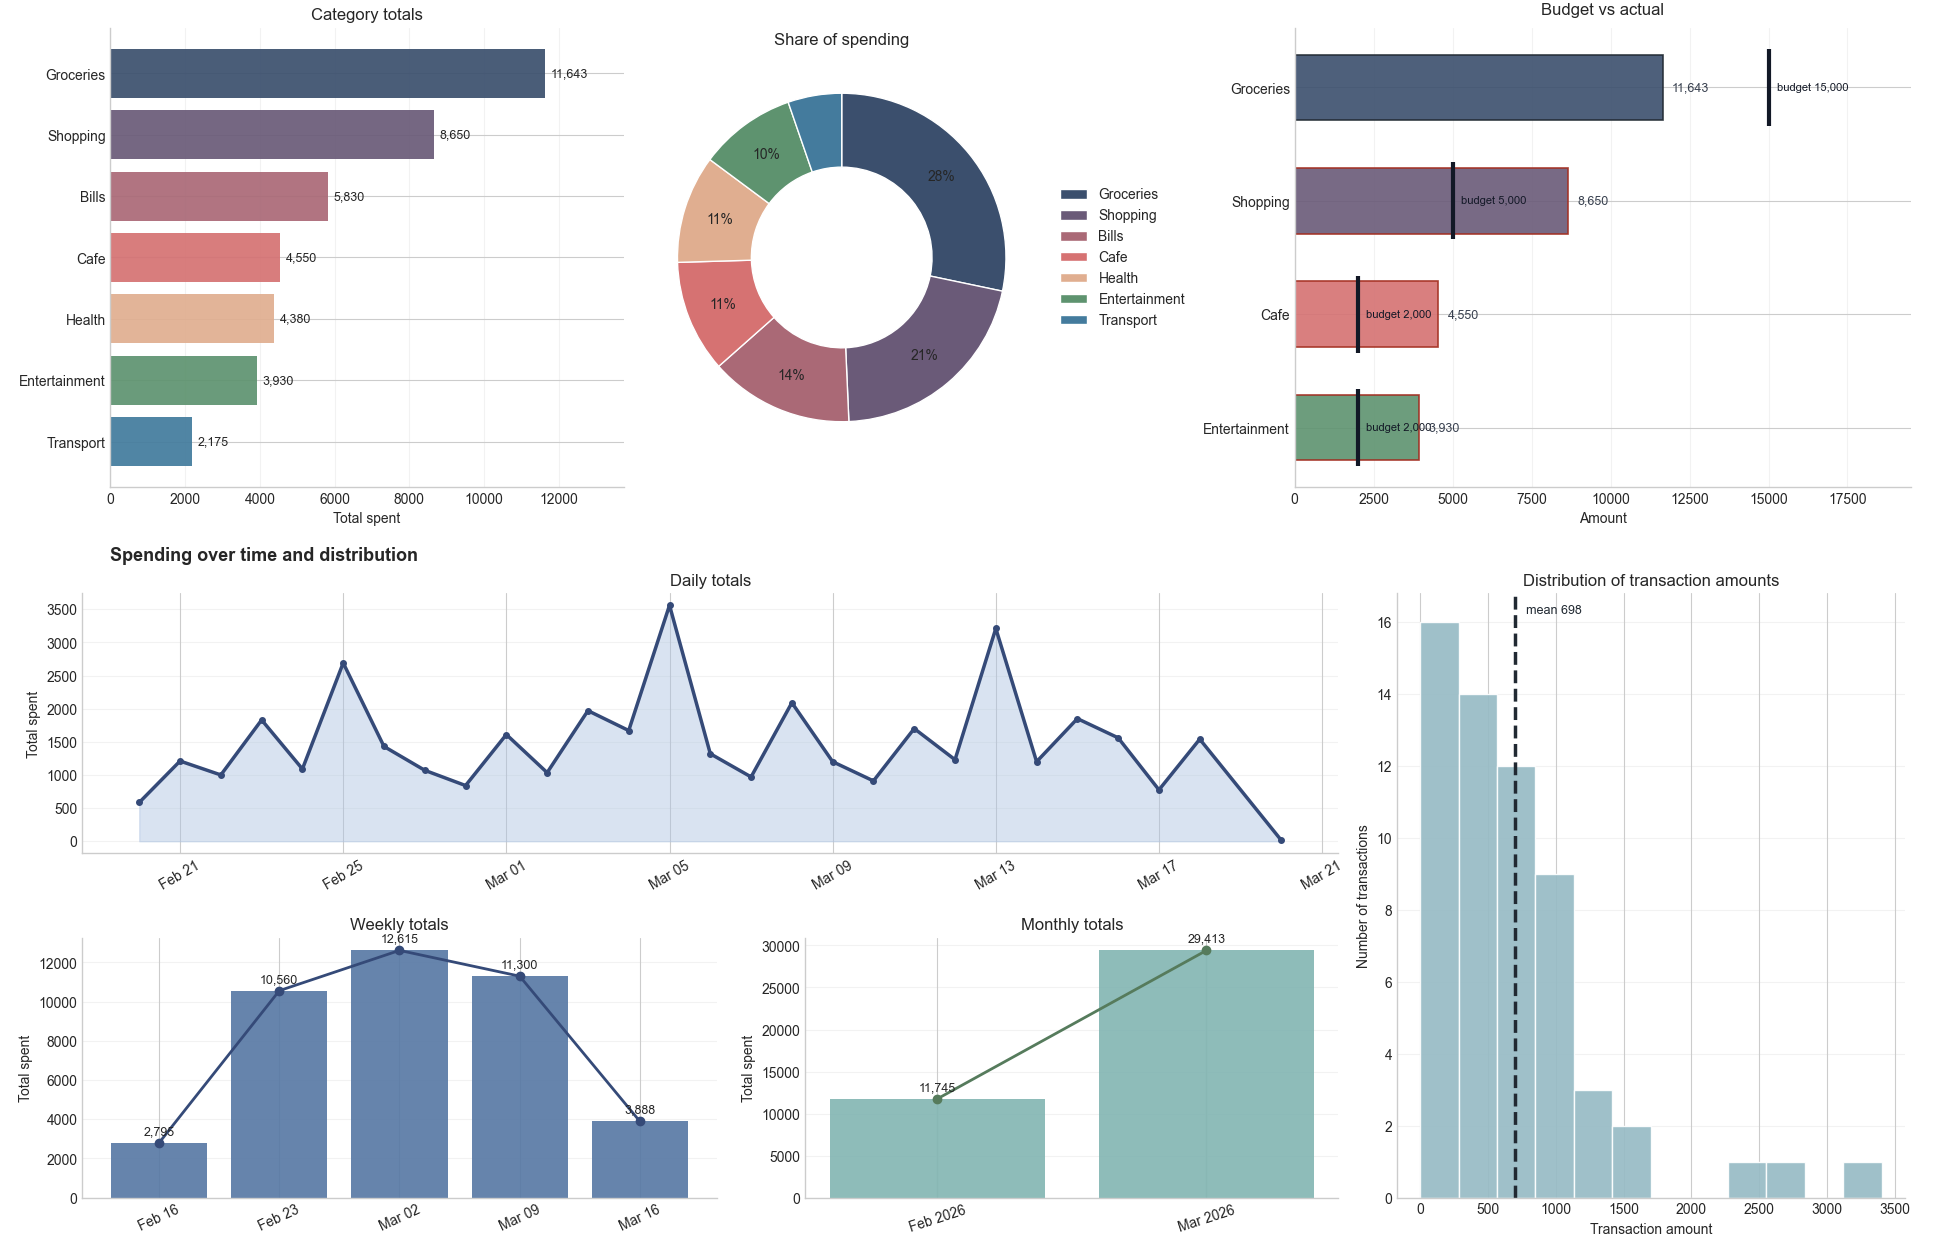
\includegraphics[width=0.98\columnwidth]{Dashboard.png}\\[-0.2em]
\scriptsize Fig. 1. Finance charts dashboard --- visualization output.
\end{center}

\begin{itemize}
\item \textbf{Month-end forecasting.} Based on the current month's spending pace, the system generates a forecast of month-end expenses. The module calculates:
\begin{itemize}
\item days elapsed in the current month and remaining days;
\item daily spending pace per category and overall;
\item projected total by category and overall at current pace;
\item projected gap compared to category budgets;
\item safe daily spending limit to stay within budget for each category.
\end{itemize}
The forecast is displayed in a table with key metrics. Categories likely to exceed the budget are highlighted. A horizontal bar chart visualizes the forecast: full bars represent projected totals, dark bars show amounts already spent, and vertical markers indicate budget limits. This feature helps users proactively adjust their spending to stay on track with financial goals. All charts are organized in a single cohesive dashboard layout with consistent color coding by category, ensuring clear visual communication of financial insights. Chart styling includes appropriate grid lines, labels, and formatting for optimal readability.
\end{itemize}

\begin{center}
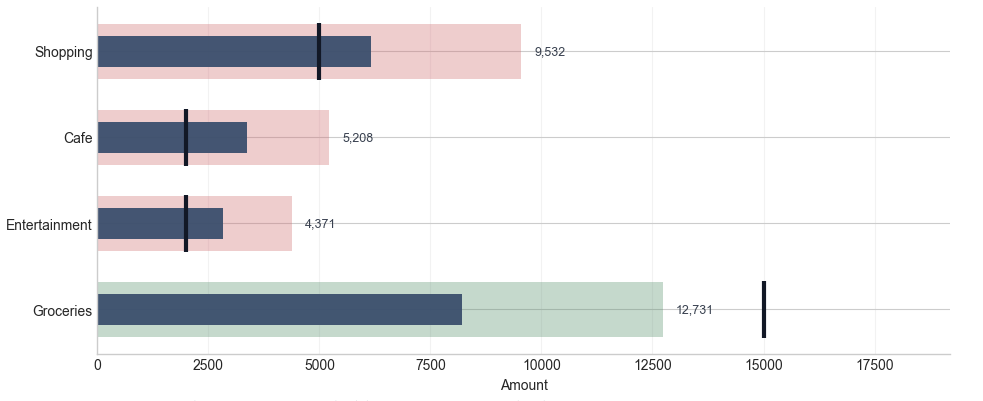
\includegraphics[width=0.95\columnwidth]{Forecast.png}\\[-0.2em]
\scriptsize Fig. 2. Month-end forecast --- chart.
\end{center}

\section{Conclusion}
During the project, a fully functional Personal Finance Tracker prototype was successfully developed and tested. The solution supports multiple data input sources: manual entry, CSV and JSON files, and automatic receipt recognition via the OCR-Space API. The system provides powerful analytical tools, including financial metrics, category and time-based grouping, budget tracking, and a comprehensive visualization dashboard. Key technical challenges included error handling for external API interactions, robust parsing of diverse receipt formats, and seamless synchronization between program modules. These were successfully addressed, resulting in a stable application with a clean modular architecture. The project has significant potential for future development: transitioning to a web application with Flask or Django, integrating with banking APIs for automatic transaction imports, applying machine learning for expense categorization and spending prediction, and developing a native mobile application. The created prototype serves as a solid foundation for a comprehensive personal financial management ecosystem.

\section*{Acknowledgement}
\begin{itemize}
\item Maria Davydova: development of the Transaction class, implementation of download functions from CSV and JSON, preparation of accounting documentation.
\item Maxim Ivanov: development of the FinanceManager class, implementation of the budget system and the \texttt{budget\_report} report, preparation of the presentation.
\item Alexey Mikhailenko: integration of the OCR module, receipt processing, and API interaction configuration.
\item Nikolay Tagin: data visualization, development of the month-end forecast module, design of final tables and graphs, implementation of the unified charts dashboard with seven chart types.
\end{itemize}

\end{document}
